\documentclass[12pt,twoside,letterpaper,onecolumn,english]{article}

\usepackage[top=1.00in, bottom=1.00in, left=1.in, right=1.in]{geometry}
\usepackage{graphicx}
\usepackage[square,numbers,sort&compress]{natbib}   % short numerical refs
\usepackage[small,compact]{titlesec}   % to squeeze the doc a bit
\setlength{\parskip}{0in}
\setlength{\parindent}{1em}
\setlength{\parsep}{0pt}
\setlength{\headsep}{0pt}
\setlength{\topskip}{0pt}
\setlength{\topmargin}{0pt}
\setlength{\topsep}{0pt}
\setlength{\partopsep}{0pt}
\setlength{\bibsep}{0.0pt}
\usepackage{hyperref}
\pdfoutput=1
\usepackage{titlesec}

\usepackage{multicol}

%\titlespacing\section{0pt}{12pt plus 4pt minus 2pt}{0pt plus 2pt minus 2pt}


\def \aap  {A\&A}
\def \aaps  {A\&AS}
\def \aj  {AJ}
\def \apj  {ApJ}
\def \apjs  {ApJS}
\def \apjl  {ApJL}
\def \apss  {AP\&SS}
\def \araa  {ARA\&A}
\def \jcap  {JCAP}
\def \prd {Phy. Rev. D}
\def \ssr {SSRv}
\def \mnras {MNRAS}
\def \nat {Nature}
\def \physrep {Phys. Rept.}
\def \pasj {PASJ}
\def \etal {et~al.~}
\def \rmxaa {RMxAA}
\def \jgr {JGR}
\def \pasp {PASP}
\def \qjras {QJRAS}

\font\myfont=cmr20 at 19pt
\font\author=cmr20 at 13pt
\font\captionf=cmr10 at 10pt


%%%%%%%%%%%%%%%%%%%%%%%%%%%%%%%%%%%%%%%%%%%%%%%%%%%%%%%%%%%%%%%%%%%%%%%%%%%%%%%%%
% a few author defined macros like:
\def\beq{\begin{equation}}
\def\eeq{\end{equation}}
%%%%%%%%%%%%%%%%%%%%%%%%%%%%%%%%%%%%%%%%%%%%%%%%%%%%%%%%%%%%%%%%%%%%%%%%%%%%%%%%%

%\title{Characterizing the Galactic population of pulsars with the {\it Fermi} Large Area Telescope.}
%\title{{\myfont Characterizing the Galactic population of pulsars with the {\it Fermi} Large Area Telescope}. \\ {\author Mattia Di Mauro, Eric Charles, Seth Digel, Matthew Wood, Regina Caputo, Paul Rey, Julia Deneva, Elizabeth Ferrara,....} }%Title in 16pt
%\author{Mattia Di Mauro, Eric Charles, Seth Digel, Matthew Wood, Regina Caputo, Paul Rey, Julia Deneva, Elizabeth Ferrara,....} 
% We don't need title or author list in the narrative
%\title{\vspace{-0.5 in}}
%\date{\vspace{-13ex}}


\begin{document}

%\maketitle

%\address{W. W. Hansen Experimental Physics Laboratory, Kavli Institute for Particle Astrophysics and Cosmology, Department of Physics and SLAC National Accelerator Laboratory, Stanford University \\
%Stanford, CA 94305, USA \\
%E-mail: mdimauro@slac.stanford.edu}


%\begin{abstract}
%\end{abstract}

%%%%%%%%%%%%%%%%% now a standard article style for the most part

\paragraph{1\ \ Scientific rationale}
\label{sec:intro}
The Large Area Telescope (LAT) on board the Gamma-Ray Space Telescope
({\it Fermi}) has been operating since 2008 producing the most detailed and precise maps of the $\gamma$-ray sky ever in the energy range $0.05-2000$~GeV.
The region toward the Galactic plane is the brighest direction in {\it Fermi}-LAT maps. $\gamma$ rays from this line of sight (l.o.s.) are mainly due to the Interstellar Emission (IE).
This is also the direction of the sky with the highest concentration of detected sources with about 70\% higher density of sources with respect to the direction outside the Galactic plane ($|b|>20^{\circ}$).

In the preliminary LAT 8-year Point Source List (FL8Y)\footnote{\url{https://fermi.gsfc.nasa.gov/ssc/data/access/lat/fl8y/}}, derived in the $0.1$-$1000$ GeV energy range, among the 2593 sources detected at $|b|<20^{\circ}$ about one half are unassociated sources.
The FL8Y contains 218 pulsars (PSR) most of which are located within a few kpc from the Solar System. These PSR belong to the disk population that follows the spiral arms of our Galaxy \cite{TheFermi-LAT:2013ssa}.
The properties of Galactic PSR emitting $\gamma$ rays, such as their luminosity function and spatial distribution, are poorly known due to detection biases and because the identification of a {\it Fermi} source as a PSR through the detection of pulsation in $\gamma$ rays is a challenging task.
The number of PSR in {\it Fermi}-LAT catalogs might be much greater because many of them could be listed among unassiciated sources due to the lack of detection of pulsation. Indeed, using the same relative numbers of FL8Y PSR and blazars, among the unassociated sources detected at $|b|<20^{\circ}$ around 220 should be PSR. 
%The identification of many more PSR with {\it Fermi}-LAT would permit to improve significantly our knowledge of the $\gamma$-ray emission mechanism, luminosity function and spatial distribution of PSR.

%namely $\gamma$ ray produced from the interaction of cosmic rays with the interstellar medium and the interstellar radiation field.
%: the interstellar emission originated from the spallation reaction of primary cosmic-ray nuclei with the interstellar gas, cosmic electrons and positrons interacting with interstellar gas and producing bremsstrahlung radiation and inverse Compton scattering of photons from interstellar radiation fields to $\gamma$-ray energies.
%In the preliminary LAT 8-year Point Source List (FL8Y)\footnote{\url{https://fermi.gsfc.nasa.gov/ssc/data/access/lat/fl8y/}}, derived in the $0.1$-$1000$ GeV energy range, among the 2593 sources detected at $|b|<20^{\circ}$: 762 are extragalactic sources (mainly blazars), 167 are pulsars (PSR) 134 are Supernovae and 1462 are unassociated. Therefore, almost one half of detected sources on the Galactic plane are unassociated. This fraction is much larger than in the extragalactic sky ($|b|>20^{\circ}$) where on average is 20-25\%. The majority of unassociated sources detected in the l.o.s of the Galactic plane are very likely from the Milky Way and most of them should be PSR. 
%Indeed, in the 3FGL 167 pulsars have been detected and the number of sources owning to this category is more than linearly increasing with the mission time (116 pulsars have been detected after 3 years).
%Associating $\gamma$-ray sources to pulsar using only the LAT data is very difficult because $\gamma$ ray pulsation needs to be measured. This is computationally extremely challenging without already knowing the value of the rotational period from radio or X-ray observations. 
%In the Second {\it Fermi} Pulsar catalog (2PC) for example over 117 sources, approximatively only one third have been discovered with blind search while two third using informations from rotational ephemerides from radio or X-ray obserservations or from radio follow-up of {\it Fermi}-LAT unassociated sources.


In the last seven years many groups analyzing
{\it Fermi}-LAT data and using  the predictions from a variety of IE models (IEM)
and point source catalogs have reported the detection of an excess at GeV
energies and $20^{\circ}$ around the Galactic center (GC) (see e.g.~\cite{TheFermi-LAT:2015kwa} and references therein).
This excess is well modeled with a spherically symmetric generalized
Navarro-Frenk-White (NFW) density profile with index $1.25$ and its
energy spectrum is peaked at a few GeV.
Recently, evidence of the existence of an unresolved population of
sources in the inner $20^\circ$ of the Galaxy with a total flux and spatial
distribution consistent with the GC excess has been published
by~\cite{Bartels:2015aea,Lee:2014mza}. These faint sources have been
interpreted as a Galactic bulge population of PSR and the brighest esemplars of this population 
should have been already detected in {\it Fermi}-LAT catalogs \cite{Cholis:2014lta}.  
The results from Refs.~\cite{Bartels:2015aea,Lee:2014mza} and the Spectral Energy Distribution (SED) 
of PSR make a Galactic bulge population of PSR one of the best motivated interpretation of this excess.

%This source population is hypothesized to be distinct from the well known disk
%population that follows the Galactic disk and its spiral arms and from
%which we detect the most local sample in radio and $\gamma$
%rays~\cite{2005AJ....129.1993M,TheFermi-LAT:2013ssa}.  

We propose to use the large amount of data collected by {\it Fermi} after almost 10 years of operation and the
huge improvement in energy and spatial resolution brought by Pass 8 \cite{2013arXiv1303.3514A} to extract from sources detected in the entire sky PSR candidates selected through criteria based on their SED.
{\bf We will use these candidates to infer for the first time the spatial distribution and luminosity function of the disk and bulge PSR population from {\it Fermi}-LAT data. 
Our list of PSR candidates will be used in radio followup search of pulsation bringing the $\gamma$-ray pulsar population to increase significantly in the next few years.
We will be able also to test the PSR interpretation of the GC excess and provide the sensitivity of the LAT to detect sources from the Galactic bulge.}





\paragraph{2\ \ Data Selection and Analysis Details}
\label{sec:details}

We plan to use ten years of Pass 8 data in an energy range $E=[0.3,500]$~GeV.
Since we are interested in detecting the emission
from point sources, we will consider {\texttt P8R2\_SOURCE\_V6} 
instrument response functions. 
%and we will select events with a maximum zenith angle of
%$90^{\circ}$ in order to minimize the contamination from the Earth atmosphere.

We are going to employ the {\texttt Fermipy} python package\footnote{See
  http://fermipy.readthedocs.io/en/latest/} that automates the analysis with {\it Fermi} Science Tools and that provides a set of high-level tools for performing $\gamma$-ray analysis such as computing SED of a source, generating Test Statistic ($TS$)\footnote{The $TS$ is defined as twice the difference in log-likelihood between the null hypothesis (i.e., no source present) and the test hypothesis: $TS = 2 \log\mathcal{L}_{\rm test} - \log\mathcal{L}_{\rm null}$} map for a region of interest, finding new source candidates, localizing a source or fitting its spatial extension.

We will search for PSR candidates using the following steps.
We subdivide the sky in Regions of Interest (ROI) each of them $12^{\circ}\times12^{\circ}$ wide.
%leaving two degrees of overlap between adjacent ROI in order to have always a good coverage for sources in the edge of an ROI. 
We will include in each ROI the IEM and isotropic template\footnote{For descriptions of these templates see http://fermi.gsfc.nasa.gov/ssc/data/access/lat/BackgroundModels.html)} and all FL8Y sources.
%with $TS>36$, since sources with a $TS = [25,36]$ could be spurious sources. 
%For the IEM and isotropic template we use the {\it gll\_iem\_v06.fits} template, released with Pass 8 data and for the isotropic component the {\it iso\_P8R2\_SOURCE\_V6\_v06.txt} template\footnote{For descriptions of these templates see http://fermi.gsfc.nasa.gov/ssc/data/access/lat/BackgroundModels.html)}. 
%Then we relocalize 3FGL sources using {\texttt Fermipy} tools since we use twice more data than in the 3FGL and the Pass 8 event selection improves significantly the spatial resolution of {\it Fermi}-LAT data.
Since we will use more data than the FL8Y, we find new sources detected with a $TS>16$.
We then make a fit to the ROI with these new seeds and we calculate SED parameters of all sources.
We plan to employ the Likelihood Weights method encoded in the {\it Fermi} Science Tools in order to include  in our analysis the uncertainties due to the modeling of the IE. 
The Galactic plane is dominated by this emission mechanism so it is of central importance to use these tools.

Finally for each source detected with $TS>25$ we will test a Power-law (PL) and Power-law with an exponential cutoff (PLE) shape for their SED\footnote{see http://fermi.gsfc.nasa.gov/ssc/data/analysis/scitools/source\_models.html for a description of the spectral models implemented in the ST}. 
From a fit to the ROI with a PL and PLE SED we will derive the likelihood value for the PL ($\mathcal{L}_{\rm{PL}}$) and PLE shapes ($\mathcal{L}_{\rm{PLE}}$) and we calculate for each source the $TS$ for a curved spectrum defined as: $TS^{\rm{PLE}}_{\rm{curv}}=2\cdot(\log{\mathcal{L}_{\rm{PLE}}} -
\log{\mathcal{L}_{\rm{PL}}})$. 
This parameter represents the preference to fit the SED of a source with a PLE with respect to a PL.
We have already applied this pipeline in \cite{Fermi-LAT:2017yoi} where we derived a catalog of sources detected in the inner $40^{\circ} \times 40^{\circ}$ region of the Galaxy. We have demostrated in that paper our capability to perform the proposed analysis.

{\bf The goal of this part of the analysis will be to have for each source the $TS$ for curvature ($TS^{\rm{PLE}}_{\rm{curv}}$), the photon index ($\Gamma$) and energy cutoff ($E_{\rm{cut}}$) in the case of PLE SED. These parameters will be used to select PSR-like sources among our list of detected sources.}




\paragraph{3\ \ Energy Spectrum of Pulsars and Blazars}
\label{sec:analysis}
In the FL8Y catalog blazars are the most numerous source
population with about 85\% of all the associated sources.
The SED of 90\% of blazars in the FL8Y are modeled with a PL function 
while blazars with a significant curvature (only about 10\% of the
entire population) are modeled with a Log-Parabola (LP).
%Blazars are divided into BL Lacertae (BL Lac) and Flat
%Spectrum Radio Quasars (FSRQ) depending on the presence or not of strong
%emission optical lines. $95\%$ of BL Lac and $85\%$ of FSRQ are modeled with a PL function
%while blazars with a significant curvature (only about 10\% of the
%entire population) are modeled with a Log-Parabola
%(LP)~\cite{Acero:2015hja}.
On the other hand of the PSR reported in FL8Y, about 80\% are
parametrized with a PLE because
they have a significant curvature and $E_{\rm{cut}}$ at a few GeV.
Thus, the shape of the energy spectrum is a promising observable that can be used to
separate PSR from blazars.

In \cite{Fermi-LAT:2017yoi} we used the 3FGL catalog to find SED-based criteria to select efficiently PSR candidates among unassociated sources.
%In the 3FGL catalog the PLE shape has not been tested for all blazars againt the LP shape.
%We can not thus use directly the 3FGL results to test PLE shape for blazars and we need to perform an SED analysis on all blazars.
We considered 7.5 years of LAT data and the analysis explained in the previous section to test the PLE versus the PL shape on blazars and PSR detected in the 3FGL with the goal of finding for each source the $TS^{\rm{PLE}}_{\rm{curv}}$, $\Gamma$ and $E_{\rm{cut}}$.
%Our sample of PSR contains 167 sources while for blazars we select sources with a significance for the curvature, as given in the 3FGL through the \texttt{Signif\_Curve} parameter, larger than 3. This cut selects 218 blazars (only 13\% of the entire sample).
We present the result of this analysis in the left panel of Fig~\ref{fig:indexcutpsrblaz} where we show the values of $\Gamma$ and $\log_{10}{(E_{\rm{cut}})}$ for blazars and PSR (divided into young and Millisecond PSR) detected with $TS^{\rm{PLE}}_{\rm{curv}}>9$.
Only 9\% of blazars have $TS^{\rm{PLE}}_{\rm{curv}}>9$ and among them only 12 have $\Gamma<2.0$ and $\log_{10}{(E_{\rm{cut}})}<4$, thus less than $1\%$ of the entire blazar population in the 3FGL catalog.
%PSR 138 16 3 TOT 157
On the other hand about 88\% of PSR have $TS^{\rm{PLE}}_{\rm{curv}}>9$ and 80\% are in this region of the PLE parameters (displayed in the figure with a cyan band). 
The average photon index and energy cutoff is $\Gamma=1.48\pm 0.45$ and $\log_{10}{(E_{\rm{cut}}[\rm{MeV}])}=3.46\pm0.25$ for young PSR and $\Gamma=1.20\pm 0.49$ and $\log_{10}{(E_{\rm{cut}}[\rm{MeV}])}=3.42\pm0.22$ for MSP. Young and MSP have thus the same energy cutoff and MSP have slightly harder indexes.
{\bf We found with 3FGL sources that the selection criteria $TS^{\rm{PLE}}_{\rm{curv}}>9$ and $\Gamma<2.0$ and $\log_{10}{(E_{\rm{cut}})}<4$ are very efficient to disentangle a PSR from a blazar. 
We plan to refine these criteria using PSR and blazars of the FL8Y and 10 years of LAT data.
We will use this SED-based selection to find PSR candidates among the sources detected in our analysis.}



\begin{figure}[t]
	\centering
	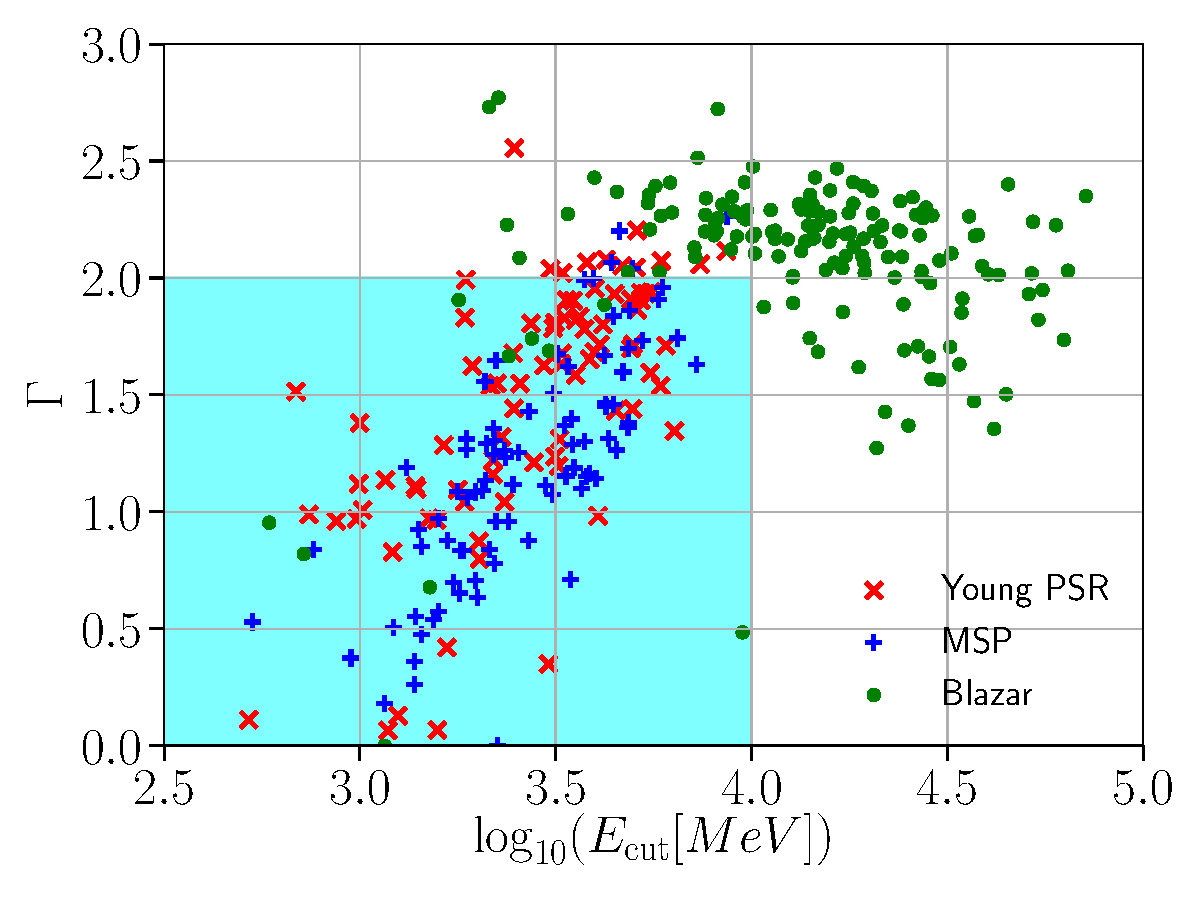
\includegraphics[width=0.49\columnwidth]{CutoffIndex_3FGL_PSRYMFSRQ_compl_TS9.pdf}
        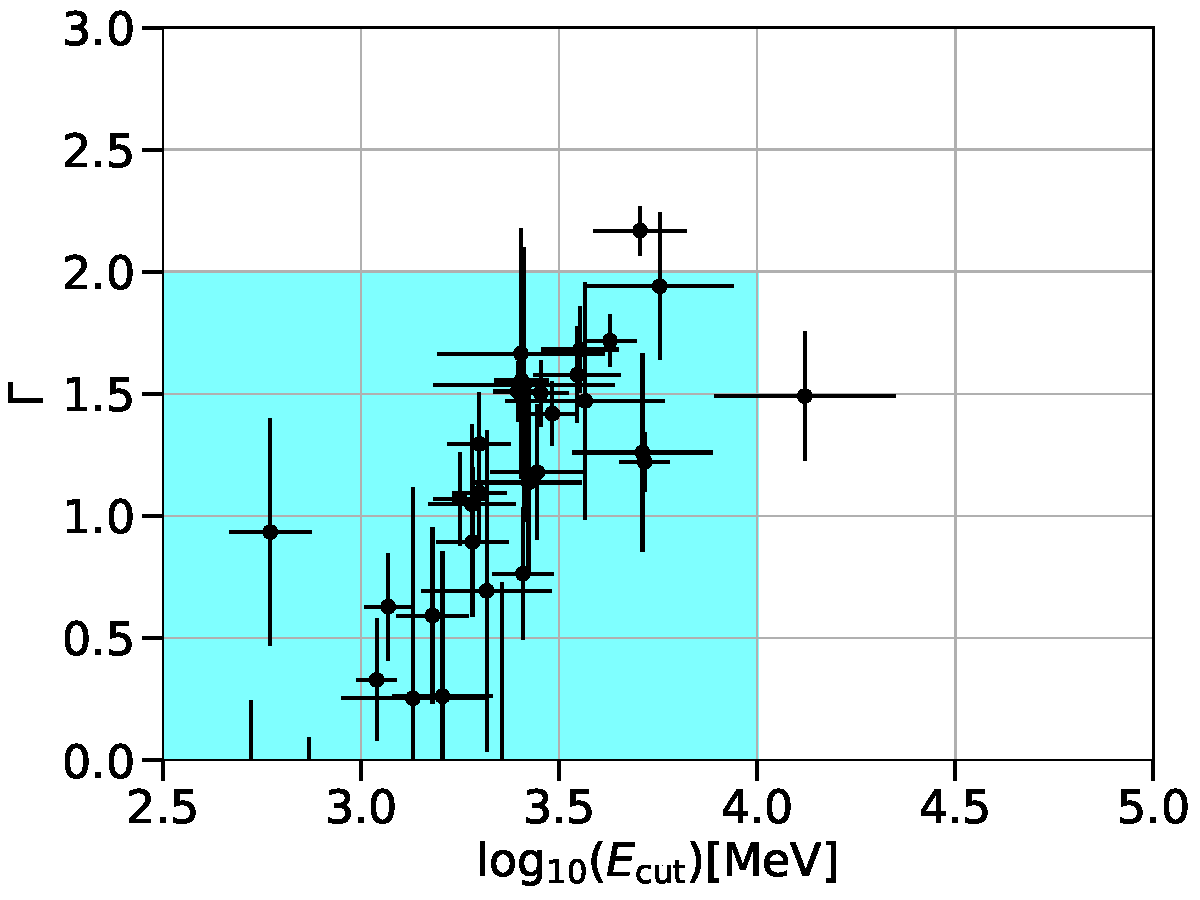
\includegraphics[width=0.49\columnwidth]{CutoffIndex_new_PSR_compl_giprop.pdf}
\vspace*{-5mm}
\caption{{\captionf Left panel: $\Gamma$ and $\log_{10}{(E_{\rm{cut}}[\rm{MeV}])}$ of 3FGL PSR (MSP are shown
  as blue points and young PSR as black points) and of blazars in the
  3FGL with $TS^{\rm{PLE}}_{\rm{curv}}>9$ (red points).  Right panel: same as in the left panel
  but for new $\gamma$-ray PSR in the FL8Y catalog.}}
\label{fig:indexcutpsrblaz} 
\end{figure}





\paragraph{4\ \ Feasibility}
We show here the feasibility of our method applying it to the most updated list of 218 $\gamma$-ray PSR in FL8Y catalog.
In particular we consider among this sample new $\gamma$-ray PSR with respect to the 3FGL.
%53 0 32 31 17 3  //  159 24 28
This selects 51 new PSR among which 26 are unassociated 3FGL sources and 25 are new sources.
We thus apply our analysis to 100 months of LAT data finding for each PSR: $TS^{\rm{PLE}}_{\rm{curv}}$, $\Gamma$ and $\log_{10}{(E_{\rm{cut}})}$ as done before for blazars and 3FGL PSR.
In the right panel of Fig.~\ref{fig:indexcutpsrblaz} we show the photon index and energy cutoff that we derive. 38 PSR over 51 have $TS^{\rm{PLE}}_{\rm{curv}}>9$ and only 2 of them has SED parameters that are not compatible with our criteria ($TS^{\rm{PLE}}_{\rm{curv}}>9$ and $\Gamma<2.0$ and $\log_{10}{(E_{\rm{cut}})}<4$).
{\bf Our method thus works very efficienctly also with new $\gamma$-ray PSR recently discovered.}

In \cite{Fermi-LAT:2017yoi} we applied the proposed analysis in the inner $40^{\circ} \times 40^{\circ}$ region of the Galaxy finding 66 sources either unassociated in the 3FGL or that are new sources and that satisfy our SED-like criteria.
These sources are therefore very promising PSR candidates.
Indeed, two of the pulsars recently discovered with {\it Fermi}-LAT data in \cite{Clark:2016unw} and that are close to the region of interest analyzed in \cite{Fermi-LAT:2017yoi} satisfy our SED-like criteria.
These sources are associated in the 3FGL with 3FGL J1650.3-4600 and 3FGL J1624.2-4041 and they have $TS^{\rm{PLE}}_{\rm{curv}}>100$ and 140, $\Gamma=1.15$ and 1.27 and $E_{\rm{cut}}=2.6$ and 2.2 GeV, respectively.
%We plan, as explained above, to make a blind search of PSR candidates among all sources detected in our analysis %calculating for them $TS^{\rm{PLE}}_{\rm{curv}}$ and PLE parameters and selecting the ones with %$TS^{\rm{PLE}}_{\rm{curv}}>9$ and $\Gamma<2.0$ and $\log_{10}{(E_{\rm{cut}})}<4$. 
%We provide here an example of our method selecting an ROI centered in $(l,b)=(-20^{\circ},-20^{\circ})$ with a width of %$12^{\circ}$. We detect 15 sources with $TS>25 $ of which 9 are 3FGL sources and 6 are new sources (see %Tab.~\ref{tab:psrcand} for their position and SED parameters). 6 sources are detected with %$TS^{\rm{PLE}}_{\rm{curv}}>9$ and among them 1 (3FGL J1730.5+0023) does not satisfies the PSR-like criteria %($E_{\rm{cut}}=21$ GeV) and in fact is a FSRQ. The other 5 sources are PSR-like source candidates and are %unassociated sources in 3FGL or new sources.
%\begin{table}[t]
%\center
%\begin{tabular}{ccccccc}
%Name & $l$[deg]        & $b$[deg]       & $TS$  &  $TS^{\rm{PLE}}_{\rm{curv}}$  &  $\Gamma$  &  $E_{\rm{cut}}$[MeV]\\
%\hline
%3FGL J1730.5+0023  &  23.8 & 18.1  &  470.8 & 16.1 & $1.92 \pm 0.11$ &  $21400 \pm 3860$ \\
%3FGL J1730.6-0357  & 19.8  &16.0  & 223 & 30.7  & $0.84 \pm  0.46$ &  $1650 \pm 540$ \\
%3FGL J1659.0-0142  & 17.6 & 23.9  &  147 & 10.3 & $0.99 \pm 0.78$ &  $3180 \pm 2600$ \\
%PS J1737.4-0317   &21.3 & 14.8  &  30 & 13.0  & $1.35 \pm  0.80$ & $1400 \pm 300$ \\
%PS J1656.5-0410  & 15.0  & 23.2  &  48 & 14.1 & $1.15 \pm 0.70$ & $1410 \pm 280$ \\
%3FGL J1653.6-0158 &  16.6 & 24.9  &  3073 & 121.2 & $1.76 \pm0.09$ &  $3200 \pm 430$ \\
%\hline
%\end{tabular}
%\caption{{\captionf Name, position, $TS$, $TS^{\rm{PLE}}_{\rm{curv}}$, $\Gamma$ and $E_{\rm{cut}}$ for sources detected with $TS^{\rm{PLE}}_{\rm{curv}}>9$.}}
%\label{tab:psrcand}
%\end{table}


\paragraph{5\ \ Efficiency and Maximum Likelihood Analysis}
We propose to employ the analysis explained above to find PSR-like sources in the entire sky. 
We will bin these detected PSR-like sources in longitude ($l$), latitude ($b$) and energy flux ($S$): $N^{\rm{real}}(l,b,S)$.
We plan then to infer the efficiency for the detection of PSR-like sources: $\omega(l,b,S)$. This will be derived simulating PSRs with different luminosities and positions in the Galaxy and using the analysis pipeline explained in this proposal to find sources detected with $TS^{\rm{PLE}}_{\rm{curv}}>9$ and $\Gamma<2.0$ and $\log_{10}{(E_{\rm{cut}})}<4$. Given the number of simulated ($N^{\rm{true}}$) and detected ($N^{\rm{det}}$) PSRs for each $l$, $b$ and $S$ bin, the efficiency is given by: $\omega(l,b,S)=N^{\rm{det}}/N^{\rm{true}}$.
We will then model the number of expected PSRs from the disk and the bulge $N_{\rm{PSR}}$. For the disk component we will start considering the spatial distribution given in \cite{2004IAUS..218..105L} while for the bulge population we will use $dN/dV\propto r^{\alpha}$ where $r$ is the radial distance from the GC \cite{Calore:2014xka}. 
The parameters of the spatial distribution of disk and bulge PSR will be free to vary in the fit.
For the luminosity of PSR we will employ a luminosity function given by a PL or a broken PL with different slopes for the disk and bulge PSR populations. 
The number of disk ($N_{\rm{disk}}$) and bulge PSR ($N_{\rm{bulge}}$) will be also free parameters. 
Given the number of PSR in our model as a function of the parameters reported above ($\vec{\lambda}$) we will calculate the number of PSR candidates detected in each pixel and energy flux bin as: $N_{\rm{PSR}}(l,b,S)=N_{\rm{PSR}}(\vec{\lambda})\times \omega(l,b,S)$. We will then employ a Maximum Likelihood Analysis (MLA) with Poisson statistics from which, comparing the number of PSR candidates from the model and from PSR candidates detected in the real sky, we will derive the best fit parameters for spatial distribution and luminosity funtcion of the disk and bulge PSR population.
{\bf This analysis will enable us to use for the first time LAT data to derive precisely the spatial distribution and luminosity function of the two PSR populations.}
%Once we have this list we will calculate with simulations the efficiency for the detection of PSR candidates as a function of longitude, latitude and energy flux $S$: $\omega(l,b,S)$. 
%The number of disk PSR $N_{\rm{disk}}$ is also free parameters of our model that need to be compatible to the number of $\gamma$-ray PSR for the disk population. 
%On the other hand the number of bulge PSR have to be consistent with a total total $\gamma$-ray intensity compatible with the $\gamma$-ray spectrum of the GC excess. 
%We have created a Python package to perform this analysis and 


\paragraph{6\ \ Plans and Schedule}
Our plan is to run our analysis {\bf in the entire sky} to find PSR-like sources (detected with $TS^{\rm{PLE}}_{\rm{curv}}>9$ and $\Gamma<2.0$ and $\log_{10}{(E_{\rm{cut}})}<4$).
We will employ the new FL8Y catalog of sources and 10 years of {\it Fermi}-LAT data.
Then we will derive the efficiency of the LAT to detect PSR-like sources and we will employ a MLA to provide predictions for the number of PSRs in the disk and in the bulge and to find their spatial distribution and luminosity function.
This result will enable us to state conclusively if the GC excess is given by a Galactic bulge PSR population.
Finally, since we demonstrated that our criteria is vey efficient in selecting PSR-like sources we are confident that we will provide PSR candidates list that could be used as targets of future radio follow for the search of radio pulsation. This will increase significantly the number of $\gamma$-ray PSRs detected by the LAT in the next few years.


{\bf Budget}: Given the substantial data analysis effort, we request one year funding to support for the PI ($\sim 30\%$), for two conferences per year and publication charges. Including overheads we request a budget of 55k\$. Co-Is Di Mauro and Charles, will be directly in charge of the analysis, while co-Is Digel and Wood will provide both technical and the scientific input.



{\footnotesize
\begin{multicols}{2}
\bibliographystyle{ieeetr}
\bibliography{psr}
\end{multicols}
}

\end{document}